\documentclass[crop,tikz,border=1px]{standalone}

\usepackage{color}
\newcommand{\red}[1]{\textcolor{red}{#1}}

\usetikzlibrary{arrows,positioning,scopes,automata,calc}

\begin{document}
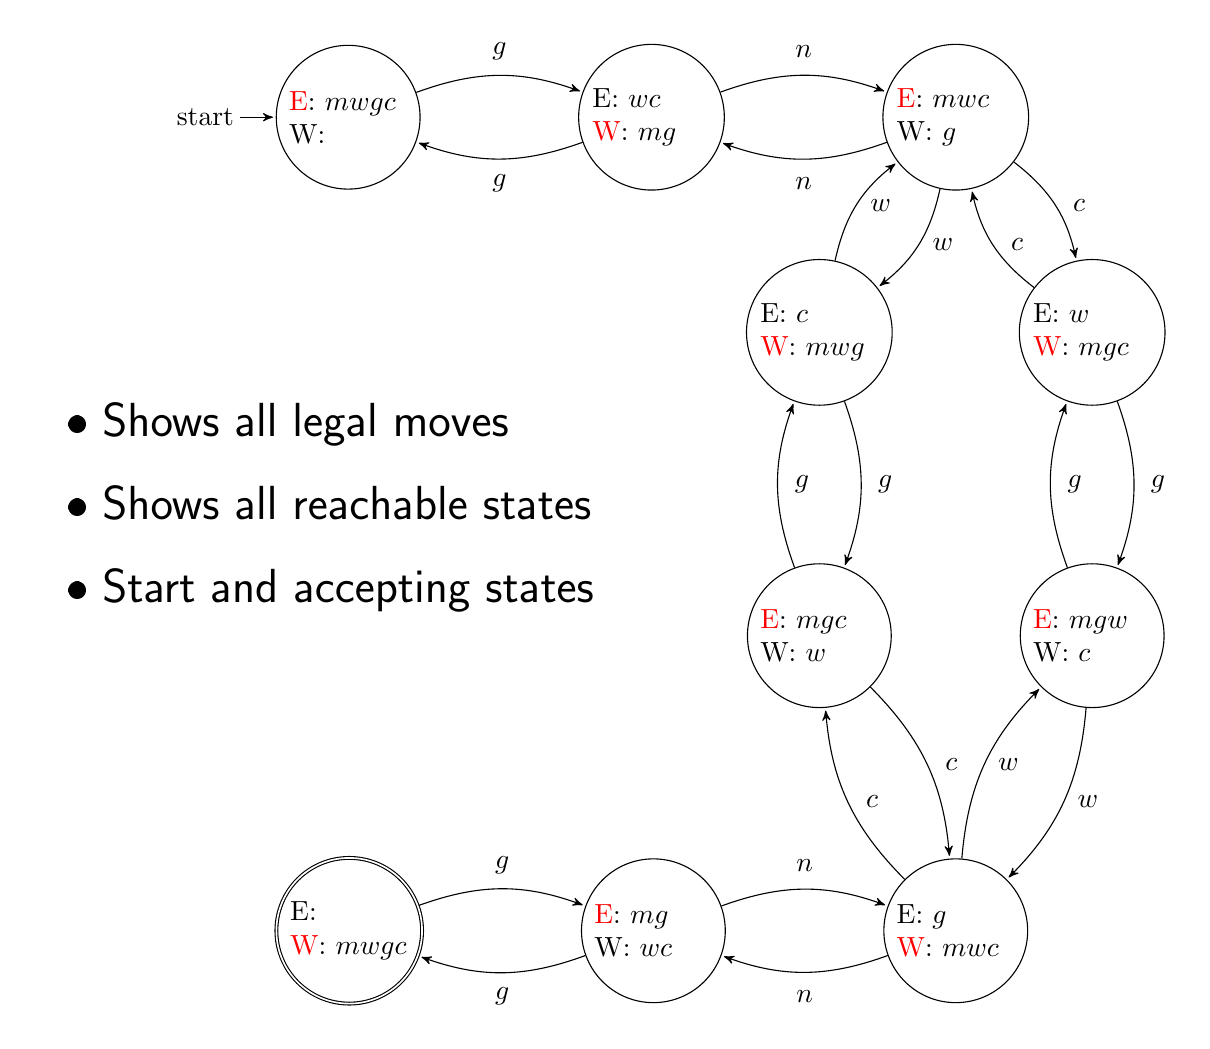
\begin{tikzpicture}[->,>=stealth',shorten >=1pt,auto,node
  distance=2cm,inner sep=2pt,minimum size=.6cm,
  mystate/.style={state,text width=1.5cm}]

  \node[initial, mystate] (s0) {\red{E}: \(mwgc\)\\W:};
  \node[mystate] (s1) [right=of s0] {E: \(wc\)\\\red{W}: \(mg\)};
  \node[mystate] (s2) [right=of s1] {\red{E}: \(mwc\)\\W: \(g\)};
  \node[mystate] (s31) [below left=of s2, xshift=1cm] {E: \(c\)\\\red{W}: \(mwg\)};
  \node[mystate] (s32) [below right=of s2, xshift=-1cm] {E: \(w\)\\\red{W}: \(mgc\)};
  \node[mystate] (s41) [below=of s31] {\red{E}: \(mgc\)\\W: \(w\)};
  \node[mystate] (s42) [below=of s32] {\red{E}: \(mgw\)\\W: \(c\)};
  \coordinate[mystate, draw=none] (mid) at ($(s41)!0.5!(s42)$);
  \node[mystate] (s5) [below=of mid] {E: \(g\)\\\red{W}: \(mwc\)};
  \node[mystate] (s6) [left=of s5] {\red{E}: \(mg\)\\W: \(wc\)};
  \node[accepting, mystate] (s7) [left=of s6] {E:\\\red{W}: \(mwgc\)};

  {[every edge/.append style={bend left=20}]
    \foreach \a/\t/\b in {s0/g/s1, s1/n/s2} {
      \path (\a) edge node [above] {\(\t\)} (\b)
            (\b) edge node [below] {\(\t\)} (\a);
    }

    \foreach \a/\t/\b in {s2/w/s31, s31/g/s41, s2/c/s32, s32/g/s42,
      s41/c/s5, s42/w/s5} {
      \path (\a) edge node [right] {\(\t\)} (\b)
            (\b) edge node [right] {\(\t\)} (\a);
    }

    \foreach \a/\t/\b in {s5/n/s6, s6/g/s7} {
      \path (\a) edge node [below] {\(\t\)} (\b)
            (\b) edge node [above] {\(\t\)} (\a);
    }
   }

   \node[draw=none, text width=8cm, below=of s0, font=\LARGE\sffamily] {
     \begin{itemize}
     \item Shows all legal moves
     \item Shows all reachable states
     \item Start and accepting states
     \end{itemize}
   };

\end{tikzpicture}
\end{document}
